\chapter{Funciones de Distancia con Signo}
\section{Introducción}
Hemos presentado anteriomente las funciones de distancia con signo como definición matemática. Ahora debemos hacernos las siguientes preguntas: ¿Cómo podemos definir \textit{funciones de distancia con signo}?, ¿qué tipo de funciones existen? y ¿qué operadores hay?.

\begin{definition}
Una función de distancia con signo, se dice exacta si está definido sobre la métrica euclídea.
\end{definition}

Vamos a definir algunas \textit{funciones de distancia con signo exactas}, que las denominaremos: \enquote{\textit{primitivas}}. En esta sección veremos primitivas sobre \(\mathbb{R}^2 \text{ y }\mathbb{R}^3\), definiéndolas centradas en el origen. Veremos también operadores para aplicar transformaciones sobre estas, como por ejemplo la traslación y la rotación.\\\\
Se ha tomado como referencia algunas primitivas propuestas por el autor, \textit{Iñigo Quilez} en su blog \enquote{\textit{Iquilezles} - Distance Functions} \url{https://www.iquilezles.org/www/articles/distfunctions2d/distfunctions2d.htm}. Aunque en su blog no se especifica ninguna demostración, se han presentado algunas demostraciones personales.

\section{Primitivas sobre \(\mathbb{R}^2\)}
En primer lugar, veremos las primitivas en \(\mathbb{R}^2\) que serán fundamentales para definir las de una dimensión superior, \(\mathbb{R}^3\). Las visualizaremos utilizando la plataforma \textit{Shadertoy}. Utilizaremos el color rojo para indicar el interior de la figura, el color azul para el exterior y el color blanco para indicar que está sobre el isoperímetro con \(\epsilon=0,01\). Crearemos líneas para ver la métrica en los diferentes puntos.
\begin{lstlisting}
#define EPSILON 0.01
void mainImage( out vec4 fragColor, in vec2 fragCoord )
{
    vec2 p = (fragCoord-iResolution.xy * 0.5)/min(iResolution.x, iResolution.y);
    // Aplicamos la FDS, f.
    float d = f(p);
    vec3 col = vec3(0.0);
    // Estamos sobre el isoperímetro.
    if(abs(d) < EPSILON){
        col = vec3(1.0);
    }else{
        if(d < 0.0){ col.x = 1.0; }
        else{ col.z = 1.0; }
    	// Número de repeticiones.
        float k = 10.0;
        col = col * (0.5 + 0.5 * (fract(abs(d) * k)));
    }
    fragColor = vec4(col, 1.);
}
\end{lstlisting}

\subsection{Circunferencia exacta}
La definición de esta figura se basa en la distancia desde cualquier punto \(\Vec{p}\) hasta \((0,0)\), el teorema de pitágoras, el módulo del vector \(\vert\vert\Vec{p}\vert\vert\)  crea una función de distancia positiva con un isoperímetro \(S=\{(0,0)\}\). Si a las distancias le restamos el radio \(r\), anularemos aquellos puntos a distancia \(r\). Cuando el vector está en el interior de la circunferencia, es decir, el módulo del vector es inferior al radio, \(\vert\vert\Vec{p}\vert\vert < r \longrightarrow \vert\vert\Vec{p}\vert\vert - r < 0\), haciendo la distancia negativa. En caso de que el módulo del vector coincide con el radio, \(\vert\vert\Vec{p}\vert\vert = r \longrightarrow \vert\vert\Vec{p}\vert\vert - r = 0\), es decir, estamos sobre el isoperímetro y finalmente, cuando módulo es mayor al radio, \(\vert\vert\Vec{p}\vert\vert > r \longrightarrow \vert\vert\Vec{p}\vert\vert - r > 0\) la distancia será positiva, en el exterior.
\begin{lstlisting}
// Circunsferencia Exacta
float SDFCircunsferencia(vec2 p, float r){
    return length(p) - r;
}
\end{lstlisting}
\begin{figure}[H]
  \centering
  \captionsetup{justification=centering}%,margin=2cm
  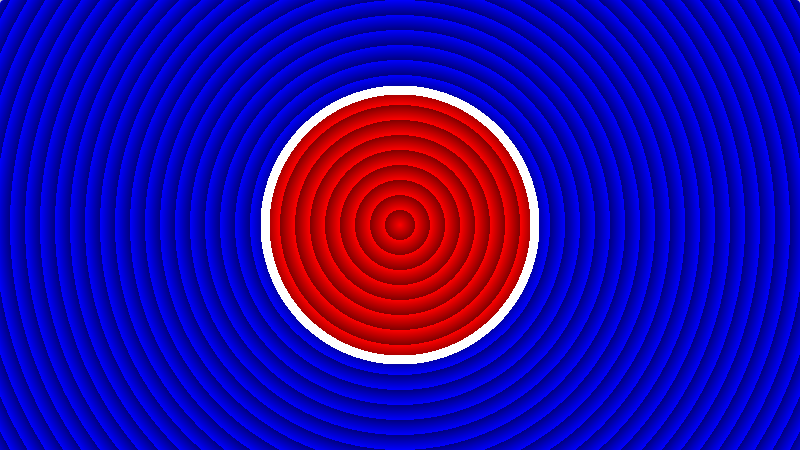
\includegraphics[width=1.0\textwidth]{secciones/imagenes/sdf/2d/sdf_circunsferencia.png}\label{fig:circ}
  \caption{Circunsferencia FDS radio \(0.3\)}
\end{figure}

% https://www.shadertoy.com/view/WtXfRj

\subsection{Rectángulo exacto}
Para calcular de forma exacta esta función vamos a definir dos operadores sobre los vectores:
\[\vert(x_0,x_1,\dots,x_n)\vert=(\vert x_0\vert,\vert x_1\vert,\dots,\vert x_n \vert)\]
\[\max\left((x_0,x_1,\dots,x_n), k\right)=(\max( x_0, k), \max(x_1, k),\dots, \max(x_n, k))\]
El operador valor absoluto es útil ya que reduce el problema a un único cuadrante, que representa un cuarto de la figura original. Las medidas serán la mitad de la original \(\Vec{s}\), en forma vectorial:
\[\Vec{s'}=(w', h')=\left(\dfrac{w}{2},\dfrac{h}{2}\right)=\dfrac{\Vec{s}}{2}\]
Situándonos en el primer cuadrante, dividimos el problema en 4 subproblemas:
\begin{figure}[H]
  \centering
  \captionsetup{justification=centering}%,margin=2cm
  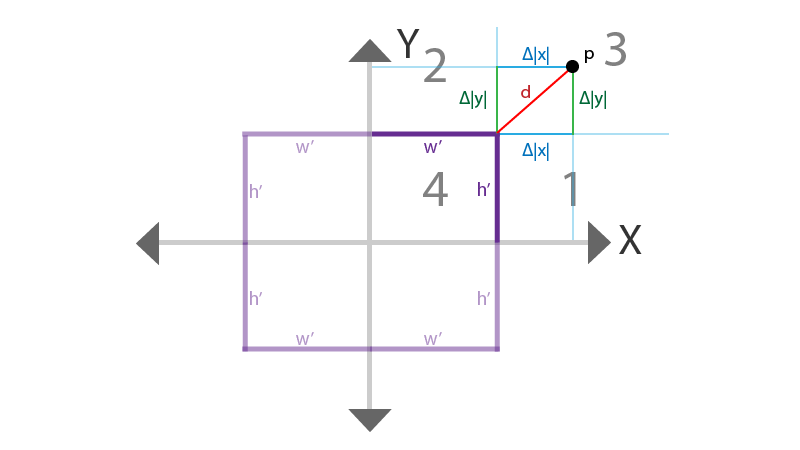
\includegraphics[width=1.0\textwidth]{secciones/imagenes/sdf/proofs/proof_rectangle.png}\label{fig:subproblem}
  \caption{División del rectángulo en 4 regiones o subproblemas.}
\end{figure}
Para cada subproblema, vamos a preservar la métrica euclídea, posicionando \(\vert\Vec{p}\vert=\vert(x,y)\vert=(\vert x\vert, \vert y \vert)\) en cada una de las regiones.
\begin{enumerate}
    \item \textbf{Región 1}. Se trata de encontrar la distancia al lado derecho, una región positiva: \(\Delta \vert x\vert=\max(\vert x\vert-w', 0)\).
    \item \textbf{Región 2}. De manera similar al anterior, la distancia al lado superior: \(\Delta\vert y\vert=\max(\vert y\vert-h', 0)\).
    \item \textbf{Región 3}. La distancia a la esquina del rectángulo, también positiva, utilizando el teorema de pitágoras: \(d = \sqrt{\left(\Delta \vert x\vert\right)^2+\left(\Delta \vert y\vert\right)^2}\).
    \item \textbf{Región 4}. La distancia en esta región es la máxima de las distancias negativas, al estar en el interior, a cada uno de los lados. Esta deberá anularse cuando nos encontremos en el exterior, definimos un nuevo operador:
    \[argmax(\Vec{a})=min(max(\Vec{a}_x, \Vec{a}_y), 0)\]
    Haciendo uso de este, la distancia interior será: \(argmax(\vert\Vec{p}\vert-\Vec{s'})\).
\end{enumerate}
Podríamos crear una función a trozos y utilizar condicionales para cada región, pero queremos que además de ser exacto, también sea eficiente, en general, las condiciones suelen ser lentas. Vamos a mirar la relación entre las diferentes regiones. Por ejemplo, observamos que la \textbf{Región 3} contiene en su ecuación a la \textbf{Región 1 y 2}, veamos casos particulares: cuando \(\Delta \vert x\vert =0\longrightarrow \sqrt{\left(\vert \Delta y\vert\right)^2} = \Delta \vert y\vert\), que concuerda con la \textbf{Región 2}, haciendo que la \textbf{Región 2 y 3} queden unificadas; Para la \textbf{Región 1 y 3}, de manera equivalente, tenemos \(\Delta \vert y\vert =0\longrightarrow \sqrt{\left(\vert \Delta x\vert\right)^2} = \Delta \vert x\vert\), vemos que la \textbf{región 3} recoge los casos para las \textbf{Regiones 1, 2 y 3}, por lo que la distancia en el exterior será
\[d_{exterior}=\vert\vert\max\left(\vert\Vec{p}\vert-\Vec{s'},0\right)\vert\vert\]
Para terminar, observamos que estamos en la \textbf{Región 4} si \(\Delta\vert x\vert \text{ y } \Delta\vert y\vert<0\), simplificándose \(d_{exterior} = 0\), por lo que bastará sumar la distancia de esta región para obtener la ecuación exacta:
\[SDFRectangulo_{\Vec{s'}}(\Vec{p})= \vert\vert\max\left(\vert\Vec{p}\vert-\Vec{s'},0\right)\vert\vert + argmax(\vert \Vec{p}\vert - {s'})\]
\begin{lstlisting}
// Rectángulo Exacto
float SDFRectangulo(vec2 p, vec2 s){
    vec2 a = abs(p) - s;
    // Exterior
    float extr = length(max(a, 0.0));
    // Interior
    float int = min(max(a.x, a.y), 0.0);
    return extr + int;
}
\end{lstlisting}
\begin{figure}[H]
  \centering
  \captionsetup{justification=centering}%,margin=2cm
  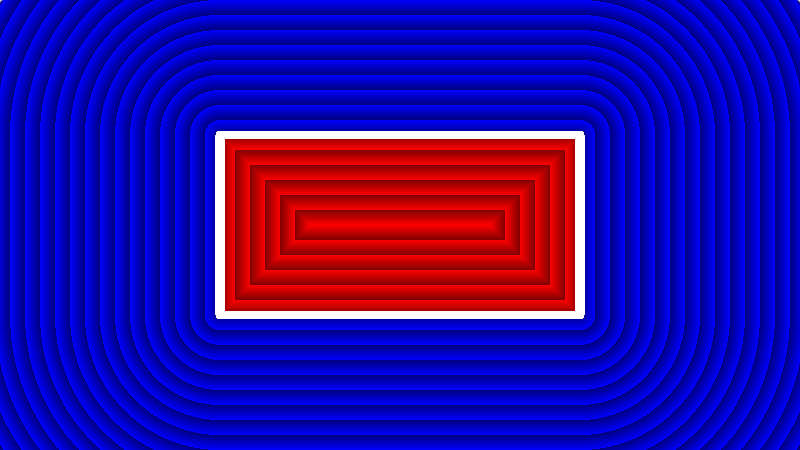
\includegraphics[width=1.0\textwidth]{secciones/imagenes/sdf/2d/sdf_rectangulo.png}\label{fig:rectaangulo}
  \caption{Rectángulo FDS de dimensiones \(\Vec{s'}=(0.4, 0.2)\)}
\end{figure}

% https://www.shadertoy.com/view/3lXBR2

\subsection{Recta exacta}
Se puede definir una recta de forma algebráica utilizando un punto y un vector director \(\Vec{n}\), para simplificar, tomaremos como punto el origen. Utilizaremos el operador de proyección\footnote{Este operador se demuestra a partir de la definición del producto escalar. Un ejemplo lo encontramos en el siguiente enlace:  \url{https://en.m.wikibooks.org/wiki/Linear_Algebra/Orthogonal_Projection_Onto_a_Line}}
para calcular el punto más cercano a la recta. El operador de proyección se define como:
\[ \text{proy}_{\Vec{n}}\Vec{p}=\left(\dfrac{\Vec{p}\cdot\Vec{n}}{\vert \Vec{n}\vert}\right)\dfrac{\Vec{n}}{\vert\Vec{n}\vert}=\left(\dfrac{\Vec{p}\cdot\Vec{n}}{\vert \Vec{n}\vert^2}\right)\Vec{n}=\left(\dfrac{\Vec{p}\cdot \Vec{n}}{\Vec{n}\cdot \Vec{n}}\right)\Vec{n}\]

\begin{figure}[H]
  \centering
  \captionsetup{justification=centering}%,margin=2cm
  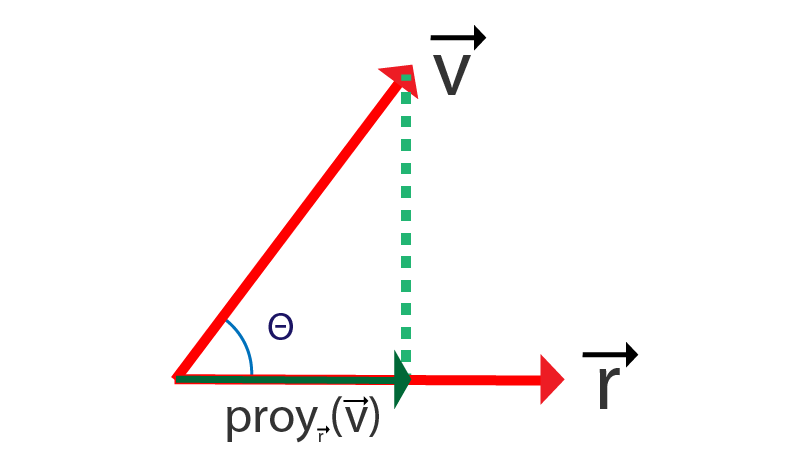
\includegraphics[width=0.8\textwidth]{secciones/imagenes/sdf/proofs/proyection.png}\label{fig:proyection}
  \caption{Proyección \(\Vec{v}\) sobre \(\Vec{r}\)}
\end{figure}

Podemos generalizar este problema para cualquier recta formada por los puntos \(\Vec{a},\Vec{b}\in\mathbb{R}^2\), cuyo vector director es 
\(\Vec{n}=\Vec{b}-\Vec{a}\). Utilizaremos uno de los dos puntos como eje de coordenadas, restando a cada punto uno de los dos vectores, por ejemplo, el vector \(\Vec{a}\) y finalmente, el resultado lo trasladamos \(\Vec{a}\). La distancia, que siempre es positiva, será la distancia del punto \(\Vec{p}\) a la proyección:
\[SDFRecta_{\Vec{a},\Vec{b}}(\Vec{p})=\vert\vert (\Vec{p}-\Vec{a}) - \text{proy}_{\Vec{p}-\Vec{a}}\left(\Vec{b}-\Vec{a}\right)\vert\vert\]

\begin{lstlisting}
// Operador Proyección a sobre b
vec2 proy(in vec2 a, in vec2 b){
    return b * dot(b, a) / dot(b, b);
}
// Línea Exacto
float SDFRecta(vec2 p, vec2 a, vec2 b){
    vec2 v = p - a;
    vec2 w = b - a;
    return length(v -  proy(v, w));
}
\end{lstlisting}
\begin{figure}[H]
  \centering
  \captionsetup{justification=centering}%,margin=2cm
  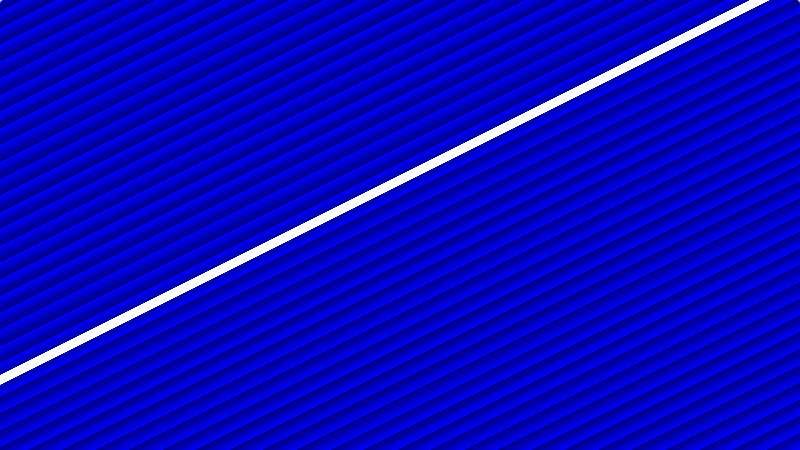
\includegraphics[width=1.0\textwidth]{secciones/imagenes/sdf/2d/sdf_recta.png}\label{fig:recta}
  \caption{FDS Recta que pasa por \(\Vec{a}=(0.2, 0.2), \Vec{b}=(0.0, 0.1)\)}
\end{figure}

% https://www.shadertoy.com/view/ttlBzX

\subsection{Segmento exacto}
Se trata de un caso particular del operador proyección entre dos vectores \(\Vec{a}, \Vec{b}\). 
\[ \text{proy}_{\Vec{b}}\Vec{a}=\left(\dfrac{\Vec{a}\cdot \Vec{b}}{\Vec{b}\cdot \Vec{b}}\right)\Vec{b}\]
Observamos que \(\dfrac{\Vec{a}\cdot \Vec{b}}{\Vec{b}\cdot \Vec{b}}\) es el factor de proyección que está en \(\mathbb{R}\). Cuando este factor es cero, la proyección será el vector \((0,0)\), en caso de que el factor tome el valor de \(1\), la proyección será el vector \(\Vec{b}\). Por lo que el segmento está formado por todos los puntos que toma el factor en el intervalo \([0,1]\):
\[ \text{proy[0,1]}_{\Vec{b}}\Vec{a}=\max\left(\min\left(\dfrac{\Vec{a}\cdot \Vec{b}}{\Vec{b}\cdot \Vec{b}}, 0\right), 1\right)\Vec{b}\]

\begin{lstlisting}
// Operador Proyección [0,1] a sobre b
vec2 proy01(in vec2 a, in vec2 b){
    return b * clamp(dot(b, a) / dot(b, b), 0., 1.);
}
// Segmento Exacto
float SDFSegmento(vec2 p, vec2 a, vec2 b){
    vec2 v = p - a;
    vec2 w = b - a;
    return length(v -  proy01(v, w));
}
\end{lstlisting}

\begin{figure}[H]
  \centering
  \captionsetup{justification=centering}%,margin=2cm
  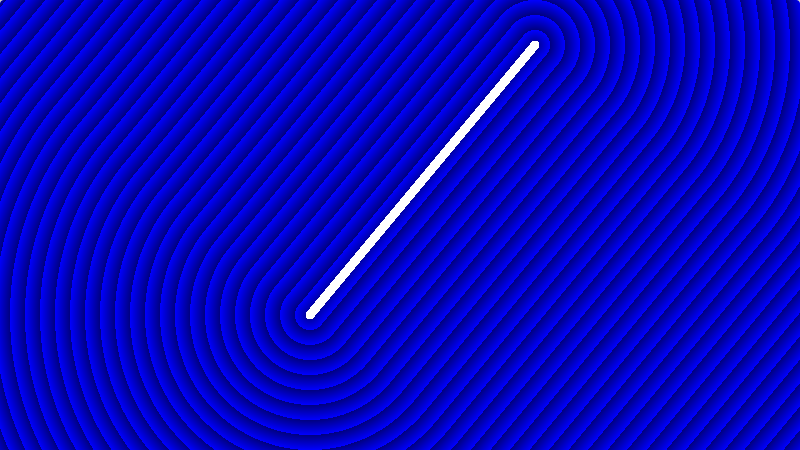
\includegraphics[width=1.0\textwidth]{secciones/imagenes/sdf/2d/sdf_segmento.png}\label{fig:segmento}
  \caption{FDS Recta que pasa por \(\Vec{a}=(-0.2, -0.2), \Vec{b}=(0.3, 0.4)\)}
\end{figure}

% https://www.shadertoy.com/view/wllBRl

Existen infinitas \textit{funciones de distancia con signo exactas}, aunque muchas no han sido propuestas debido a su complejidad. Vamos a presentar operadores que nos van a ayudar a transformar estas funciones, resultando de otras que pueden o no preservar la \textit{exactitud}. La exactitud provocará modificaciones en algunos de los algoritmos, principalmente sobre \(\mathbb{R}^3\).\\\\
Podemos encontrar más \textit{funciones de distancia con signo exactas} en el siguiente enlace: \url{https://www.iquilezles.org/www/articles/distfunctions2d/distfunctions2d.htm}, aunque no sus demostraciones. Muchas de estas pueden ser demostradas utilizando las propiedades y operadores vistos en los apartados anteriores, por ejemplo, la definición exacta del triángulo hace uso de dos segmentos para dos de sus lados conectados por una arista y las coordenadas baricéntricas\footnote{El sistema de coordenadas baricéntrico se generar a partir del baricentro, es decir, el punto de corte de las tres rectas que pasan por el centro de un lado y por el vértice opuesto. Podemos encontrar la demostración de la distancia en el siguiente enlace: \url{https://mathoverflow.net/a/36669}}.

\section{Operadores sobre \(\mathbb{R}^2\)}
Vamos a ver operadores imprescindibles para poder manipular nuestra escena, además de poder crear nuevas \textit{funciones de distancia con signo exactas}. Estos operadores pueden preservar o no la exactitud de nuestras funciones, aquellos operadores que la preserven, los llamaremos \textit{isometrías}.

\begin{definition}
Una aplicación \(g\) sobre dos espacios métricos se dice que es \textit{isométrica} si se conservan la distancia entre todos los puntos antes y después de su aplicación. \[\forall \Vec{v},\Vec{w} \in\mathbb{R}^2, d(\Vec{v},\Vec{w})=d(g(\Vec{v}),g(\Vec{w}))\]
\end{definition}

En secciones anteriores hemos visto por qué vamos a trabajar sobre la métrica euclídea, esto implicará que la función de distancia \(d\), sea  \(d(\Vec{v},\Vec{w})=d((x,y),(z,w))=\vert\vert \Vec{v}-\Vec{w}\vert\vert=\sqrt{(x-z)^2+(y-w)^2}\). En la siguiente sección veremos tres \textit{isometrías}: la traslación, la rotación y la simetría sobre una recta.

\subsection{Operador de traslación}
Definimos la traslación como el operador donde un punto \(\Vec{p}\) es desplazado por un vector \(\Vec{t}\), preservando las características:
\[\text{traslacion}(\Vec{p},\Vec{t})=\Vec{p}\pm\Vec{t}\]
Vamos a demostrar que la traslación es una isometría, \(\forall \Vec{v},\Vec{w}\in\mathbb{R}^2\):
\[d(f(\Vec{v}), f(\Vec{w}))=d(\Vec{v}\pm\Vec{t}, \Vec{w}\pm\Vec{t})=\vert\vert (\Vec{v}\pm\Vec{t})-(\Vec{w}\pm\Vec{t})\vert\vert=\vert\vert \Vec{v}-\Vec{w}\vert\vert=d(\Vec{v}, \Vec{w})\]
Este es uno de los motivos por el cual se ha definido las \textit{funciones de distancia con signo} sobre el origen. Por fin, podemos trasladarlo a cualquier parte de nuestra escena, en código:
\begin{lstlisting}
float escena_sdf(vec2 p){
    // Trasladamos el vector p hacia 0.1 izquierda y 0.2 a la derecha.
    vec2 pt = p - vec2(0.1, 0.2);
    return SDFCircunsferencia(pt, 0.3);
}
\end{lstlisting}

Hemos realizado una resta en vez de una suma para trasladarlo a la posición deseada. Aunque parece contraintuitivo, debemos imaginarlo como si nuestros ojos estuvieran sobre el plano, cambiado las orientaciones.

\begin{figure}[H]
  \centering
  \captionsetup{justification=centering}%,margin=2cm
  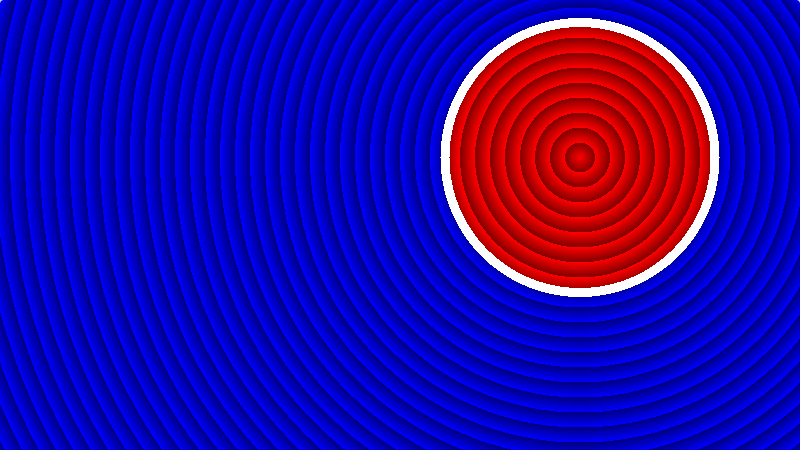
\includegraphics[width=1.0\textwidth]{secciones/imagenes/sdf/2d/sdf_traslacion.png}\label{fig:traslacion}
  \caption{Traslación FDS \(\Vec{t}=(0.1, 0.2)\)}
\end{figure}

% https://www.shadertoy.com/view/ttXfWS

\subsection{Operador de rotación}
El segundo operador que vamos a presentar es el operador de rotación. Se define como la matriz de rotación\footnote{Esta matriz es definida por el mapeo de coordenadas polares y la linearidad. La demostración la encontramos en el siguiente enlace: \url{https://math.stackexchange.com/a/53181}}, donde \(\alpha\) es el ángulo de rotación en radianes y es una matriz ortogonal\footnote{Una matriz se dice ortogonal, si y solo si, \(A\cdot A^t=I\). La demostración de que la matriz de rotación es ortogonal:  \url{https://math.stackexchange.com/a/2471175}}:
\[ 
\text{rot}(\alpha)=\begin{pmatrix}
    +\cos(\alpha) & -\sin(\alpha)\\
    +\sin(\alpha) & +\cos(\alpha)
\end{pmatrix}
\]
que aplicada sobe un vector \(\Vec{p}=\begin{pmatrix}
    x\\
    y
\end{pmatrix}\),
\[ 
\text{rotacion}_\alpha(\Vec{p})=\Vec{p}\cdot\text{rot}(\alpha)=\begin{pmatrix}
    x\\
    y
\end{pmatrix}^t\cdot\begin{pmatrix}
    +\cos(\alpha) & -\sin(\alpha)\\
    +\sin(\alpha) & +\cos(\alpha)
\end{pmatrix}
\]
Resultando,
\[\text{rotacion}_\alpha(\Vec{p})=\begin{pmatrix}
    +x\cos(\alpha) + y\sin(\alpha)\\
    -x\sin(\alpha) + y\cos(\alpha)
\end{pmatrix}
\]
Veamos que el operador también es una \textit{isometría}, \(\forall \Vec{v},\Vec{w}\in\mathbb{R}^2\):
\[d(f(\Vec{v}), f(\Vec{w}))=d(\Vec{v}\cdot \text{rot}(\alpha), \Vec{w}\cdot \text{rot}(\alpha))=\]\[\vert\vert \Vec{v}\cdot \text{rot}(\alpha)- \Vec{w}\cdot \text{rot}(\alpha)\vert\vert=\vert\vert(\Vec{v}-\Vec{w})\cdot \text{rot}(\alpha)\vert\vert\]
Como \(\text{rot}(\alpha)\) es ortogonal: \(\vert\vert A\cdot\text{rot}(\alpha)\vert\vert=\vert\vert A\vert\vert\).\footnote{La demostración de esta propiedad requiere un alto conocimiento matemático, como curiosidad, encontramos la demostración en el siguiente enlace: \url{https://math.stackexchange.com/a/2245861}}
\[d(f(\Vec{v}), f(\Vec{w}))=\vert\vert(\Vec{v}-\Vec{w})\cdot \text{rot}(\alpha)\vert\vert=\vert\vert\Vec{v}-\Vec{w})\vert\vert=d(\Vec{v},\Vec{w})\]
En código,
\begin{lstlisting}
#define PI 3.1415
mat2 rot(float a){
    return mat2(
        +cos(a), -sin(a), 
        +sin(a), +cos(a)
    );
}
// Escena
float escena_sdf(vec2 p){
    // Rotacion del el vector p 45 grados o pi / 4 radianes.
    vec2 pr = p * rot(45. * PI / 180.);
    return SDFRectangulo(pr, vec2(0.3));
}
\end{lstlisting}

\begin{figure}[H]
  \centering
  \captionsetup{justification=centering}%,margin=2cm
  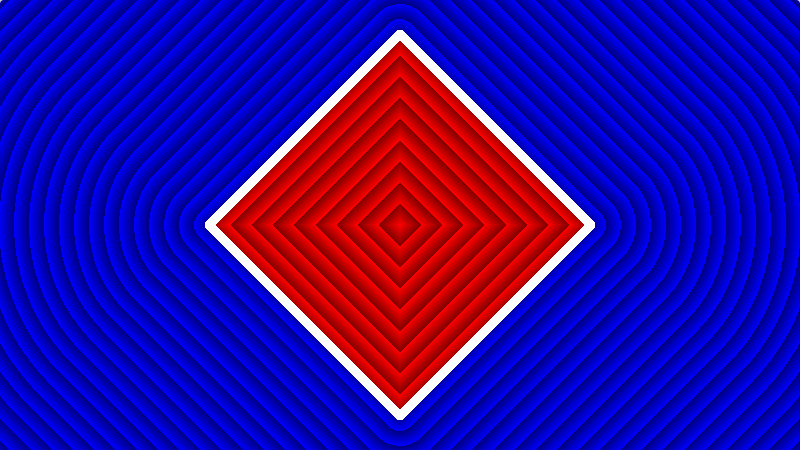
\includegraphics[width=1.0\textwidth]{secciones/imagenes/sdf/2d/sdf_rotacion.png}\label{fig:rotacion}
  \caption{Rectángulo (cuadrado) FDS con rotación \(\alpha=\dfrac{\pi}{4}\)}
\end{figure}

% https://www.shadertoy.com/view/wlXfDS

\subsection{Operador de simetría}
La simetría traslada los puntos que están sobre un lado de la recta hasta el otro lado tal que estos equidisten.\\\\ Dado un vector director \(\Vec{n}\in\mathbb{R}^2\) de una recta que pasa por el \((0,0)\) y utilizando el operador de proyección de cualquier punto \(\Vec{p}\in\mathbb{R}^2\) sobre \(\Vec{n}\). La simetría consiste en trasladar \(\Vec{p}\) hacia el otro lado de la recta en dirección al punto proyectado.
\[\text{simetria}_{\Vec{n}}(\Vec{p})=\Vec{p} + 2(\text{proy}_{\Vec{n}}(\Vec{p})-\Vec{p})\]
Para cualquier recta formada por dos puntos \(\Vec{a}, \Vec{b}\), el operador de simetría será:
\[\text{simetria}_{\Vec{a},\Vec{b}}(\Vec{p}) =\Vec{a}+ \text{simetria}_{\Vec{b}-\Vec{a}}(\Vec{p}-\Vec{a})\]
Veamos algunos casos particulares, los definidos sobre los ejes:\\\\
Sobre el eje \(X\), \(\Vec{n}=(1,0)\), definimos el operador de simetría sobre el eje x como
\[\text{simetria}_{X}(\Vec{p})=\text{simetria}_{\Vec{n}}(\Vec{p})=(-x, y)\]
De manera equivalente para el eje \(Y\):
\[\text{simetria}_{Y}(\Vec{p})=\text{simetria}_{\Vec{n}}(\Vec{p})=(x, -y)\]
Se deja una cuestión abierta sobre estos dos últimos operadores de simetría. ¿Qué ocurriría si \enquote{dobláramos} el eje y?, es decir:
\[\text{simetria}_{\vert Y\vert}(\Vec{p})=\text{simetria}_{\Vec{n}}(\Vec{p})=(x, -\vert y\vert)\]


\newpage
Veamos la definición en código,
\begin{lstlisting}
// Simetría sobre el origen
vec2 simetria(vec2 n, vec2 p){
    return p + 2. * (proy(p, n) - p);
}
// Sobre cualquier recta genérica formada que pasa por a y b.
vec2 simetria(vec2 p, vec2 a, vec2 b){
    return a + simetria(b - a, p - a);
}
\end{lstlisting}
Veamos el ejemplo en práctica sobre la recta definida en \fullref{fig:recta} con la función de distancia con signo definida en \fullref{fig:segmento}.
\begin{lstlisting}
float escena_sdf(vec2 p){
    // Recta Simetría
    vec2 a = vec2(0.2, 0.2);
    vec2 b = vec2(0.0, 0.1);
    // Simetría
    vec2 ps = simetria(p, a, b);
    
    return SDFSegmento(
        ps,
        vec2(-0.2, -0.2), 
        vec2(0.3, 0.4)
    );
}
\end{lstlisting}

\begin{figure}[H]
  \centering
  \captionsetup{justification=centering}%,margin=2cm
  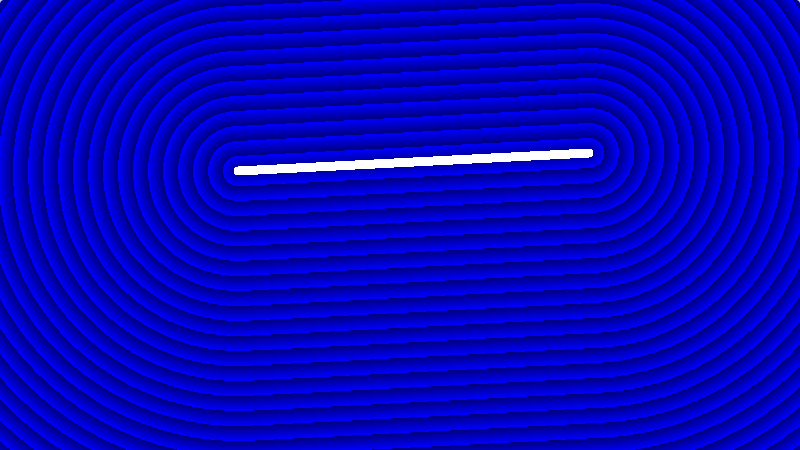
\includegraphics[width=1.0\textwidth]{secciones/imagenes/sdf/2d/sdf_simetria.png}\label{fig:simetria}
  \caption{Simetría FDS ejemplos anteriores}
\end{figure}

% https://www.shadertoy.com/view/3lsBWS

Veamos ahora algunos operadores entre \textit{funciones de distancia con signo}. Estos operadores van a ser vitales para crear escenas complejas, ya que van a permitir agregar o sustraer \textit{funciones de distancia con signo exactas}.

\subsection{Operador de agregación}
Ya vista la función de traslación, ahora nos puede ser útil ver como agregar dos \textit{funciones de distancia con signo}. El resultado de este operador será otra \textit{función de distancia con signo} formado por la distancia menor en cada punto de las dos funciones a agregar. Esta descripción se define como:
\[\text{Agregacion}(\Vec{p}, f, g) = \min(f(\Vec{p}), g(\Vec{p})) \]
Utilizaremos la función \enquote{\textit{min}} que está definida en el lenguaje \textit{GLSL}. Veamos un ejemplo, utilizaremos los dos últimos ejemplos de \textit{isometrías}, la traslación \fullref{fig:traslacion} y la rotación \fullref{fig:rotacion}:
\begin{lstlisting}
// Escena
float escena_sdf(vec2 p){
    // Rotamos el rectángulo 45 grados - f
    vec2 pr = p * rot(PI / 180. * 45.0);
    // Trasladamos el rectangulo hacia 0.1 - g izquierda y 0.2 a la derecha.
    vec2 pt = p - vec2(0.4, 0.15);
    // Unión de dos FDS
    return min(
        SDFRectangulo(pr, vec2(0.3)), // f
        SDFCircunsferencia(pt, 0.3)   // g
    );
}
\end{lstlisting}

El resultado de la adición es el siguiente:

\begin{figure}[H]
  \centering
  \captionsetup{justification=centering}%,margin=2cm
  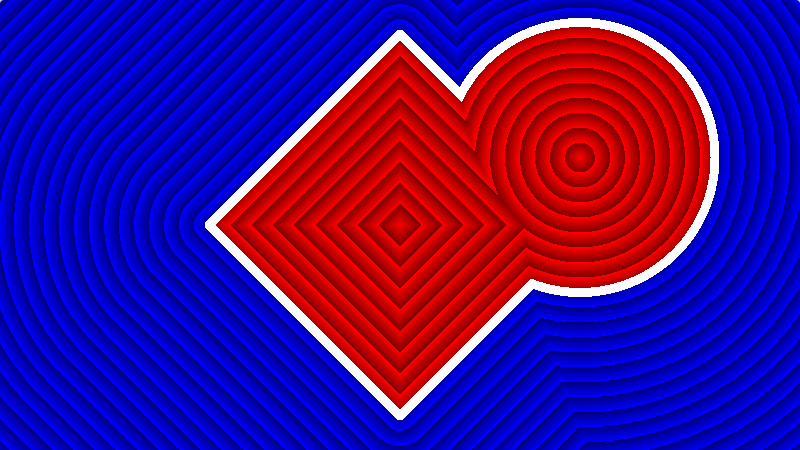
\includegraphics[width=1.0\textwidth]{secciones/imagenes/sdf/2d/sdf_add.png}\label{fig:add}
  \caption{ Adición de dos FDS de ejemplos anteriores}
\end{figure}

% https://www.shadertoy.com/view/WlsBDS

Como el resultado también es una \textit{función de distancia con signo}, podemos componer estos operadores.
\subsection{Operador de substracción}
Antes hemos visto que el operador \enquote{\(\min\)} que combina dos \textit{FDS}, podemos imaginarnos que hace el operador \enquote{\(\max\)}. Este devuelve la distancia más lejana entre las dos, es decir, devuelve la intersección de ambos, ya que si alguna distancia es positiva, devolverá siempre la positiva, en caso de ambas ser negativas, devolverá la menor.

\begin{figure}[H]
  \centering
  \captionsetup{justification=centering}%,margin=2cm
  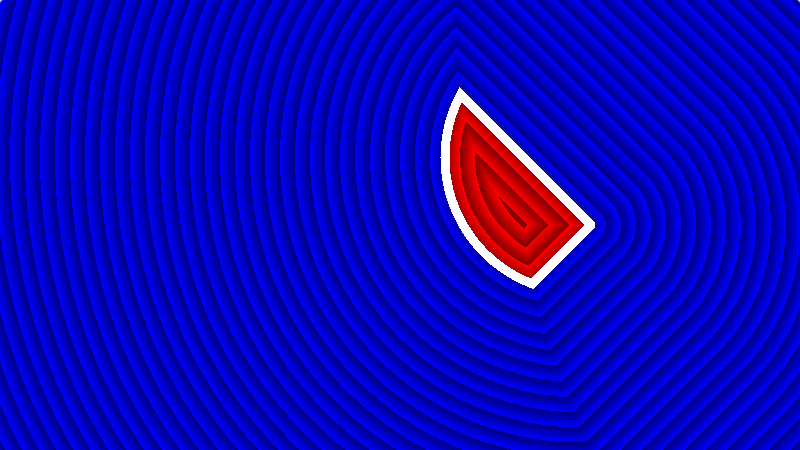
\includegraphics[width=0.8\textwidth]{secciones/imagenes/sdf/2d/sdf_subtract-1.png}\label{fig:disyunccion}
  \caption{Intersección de las dos FDS de ejemplos anteriores}
\end{figure}

% https://www.shadertoy.com/view/3llfDS

Vamos a crear el operador de substracción, utilizando el de intersección, pero antes, es fácil observar que podemos cambiar el interior por el exterior, que llamarermos inversión de una \textit{función de distancia con signo}. Bastaría con cambiar el signo, multiplicando por \(-1\).
\[ Inversión(\Vec{p}, f) = -f(\Vec{p}) \]

\begin{figure}[H]
  \centering
  \captionsetup{justification=centering}%,margin=2cm
  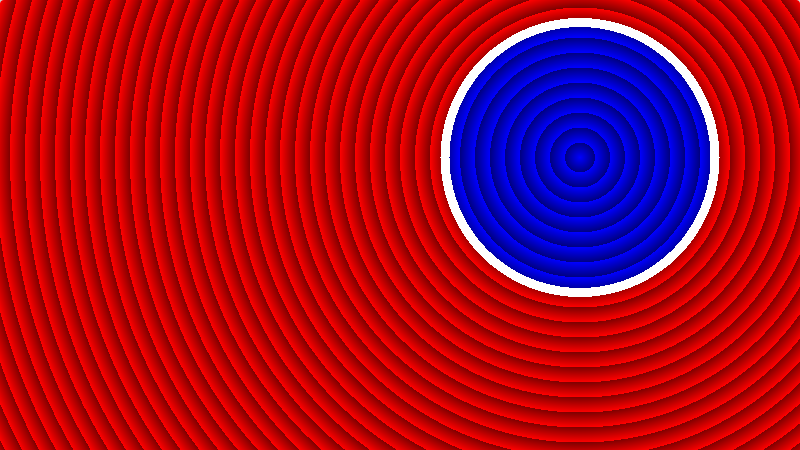
\includegraphics[width=1.0\textwidth]{secciones/imagenes/sdf/2d/sdf_subtract-2.png}\label{fig:negative}
  \caption{ Interior por Exterior Circunsferencia FDS}
\end{figure}

% https://www.shadertoy.com/view/WlsfDS

Ahora, las distancias negativas representan el exterior de la figura anterior. Esto junto a la definición de intersección, se eliminará de una figura el interior de la figura anterior. Definimos la substracción de una función de distancia con signo \(f\) otra \(g\), tal que:
\[\text{substraccion}(\Vec{p}, f,g)=max(f(\Vec{p}), -g(\Vec{p}))\]
Un ejemplo en código:
\begin{lstlisting}
float escena_sdf(vec2 p){
    // Rotamos el rectángulo 45 grados
    vec2 pr = p * rot(PI / 180. * 45.0);
    
    // Trasladamos la circunferencia
    vec2 pt = p - vec2(0.4, 0.15);
    // Sustraemos Una circunsferencia de un rectángulo.
    return max(
        SDFRectangulo(pr, vec2(0.3)),
        -SDFCircunsferencia(pt, 0.3)
    );
}
\end{lstlisting}
El resultado de la ejecución del código:
\begin{figure}[H]
  \centering
  \captionsetup{justification=centering}%,margin=2cm
  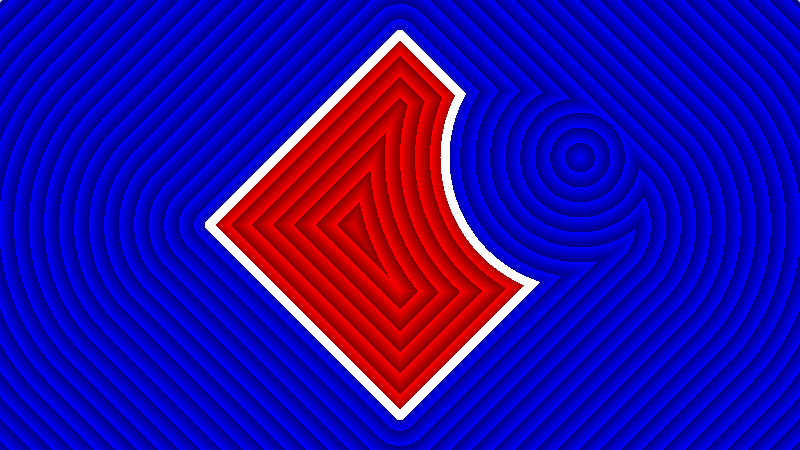
\includegraphics[width=1.0\textwidth]{secciones/imagenes/sdf/2d/sdf_subtract-3.png}\label{fig:substraction}
  \caption{Substracción de una circunsferencia a un rectangulo FDS}
\end{figure}

% https://www.shadertoy.com/view/WllBWB

%Cabe destacar que esta figura no preserva las distancias, por lo que el objeto restado tendrá el espacio distorsionado, veremos en los siguientes capítulos, como solucionarlo.\\\\
Vamos a ver otro tipo de transformaciones, las que manipulan el espacio, esto puede hacer que el resultado de las funciones no sean exacto o que debamos hacer una transformación que las transforme en exactas, por ejemplo, el escalado.

\subsection{Operador de escalado}
Veamos como escalar una función de distancia con signo y como podemos solucionar esta deformación. Supongamos que el escalado fuera una isometría, es decir:
\[g(\Vec{p})=\Vec{p}\cdot \dfrac{1}{k}, k \in \mathbb{R}^{+}_{0}\]
Donde \(k\) es el factor de escalado, veamos que no es una isometría y como lo solucionamos, \(\Vec{v},\Vec{w}\in \mathbb{R}^2\).
\[d(g(\Vec{v}),g(\Vec{w}))=d\left(\Vec{v}\cdot \dfrac{1}{k}, \Vec{w}\cdot \dfrac{1}{k}\right) = \vert\vert \Vec{v}\cdot \dfrac{1}{k} - \Vec{w}\cdot \dfrac{1}{k}\vert\vert=\vert\vert (\Vec{v} - \Vec{w})\cdot \dfrac{1}{k}\vert\vert\]
Vemos que la distancia transformada es proporcional a la distancia inicial con factor \(\dfrac{1}{k}\). Para solucionar esto, multiplicamos la distancia por el factor \(k\), esto hará que el factor se cancele, consiguiendo así una isometría.\\\\
Según los valores que tome \(k\): cuando \(k<1\), estamos reduciendo el tamaño; si \(k=1\) el tamaño original se preserva y finalmente, con \(k>1\) agrandamos.\\\\
Veamos un ejemplo, por ejemplo, escalamos el ejemplo anterior con un factor de \(k=0.5\), reduciendo a la mitad:
\begin{lstlisting}
float escena_sdf(vec2 p){
    // Factor de escalado
    float k = 0.5;
    // Escalamos todas las figuras
    p = p / k;
    // Rotamos el rectángulo
    vec2 pr = p * rot(PI / 180. * 45.0);
    // Trasladamos la circunferencia
    vec2 pt = p - vec2(0.4, 0.15);
    float d = max(
        SDFRectangulo(pr, vec2(0.3)),
        -SDFCircunsferencia(pt, 0.3)
    );
    // Multiplicamos por la distancia para hacerlo una isometría.
    return d * k;
}
\end{lstlisting}

El resultado del escalado es el siguiente:

\begin{figure}[H]
  \centering
  \captionsetup{justification=centering}%,margin=2cm
  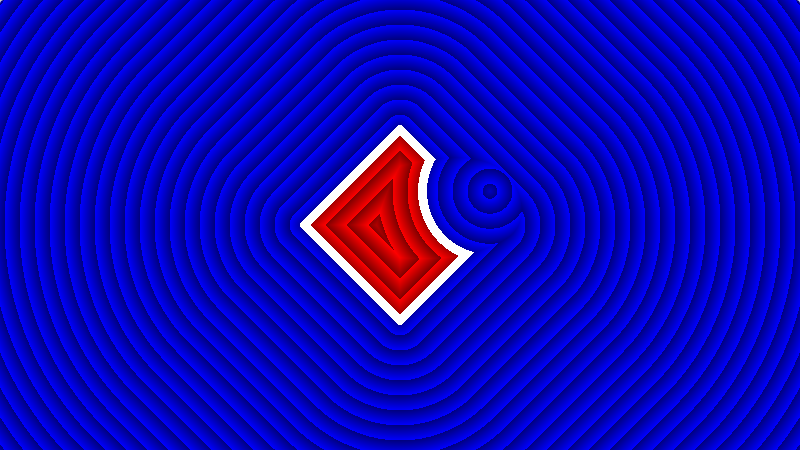
\includegraphics[width=1.0\textwidth]{secciones/imagenes/sdf/2d/sdf_subtracted_scale.png}\label{fig:substraction}
  \caption{Ejemplo anterior escalado con \(k=0.5\)}
\end{figure}

% https://www.shadertoy.com/view/WlsBDX

\subsection{Operador de deformación sin exactitud}
Como se ha comentado antes, hay deformaciones que no preservan la métrica y por tanto las funciones no son exactas. En general, consiste en aplicar una función no \textit{isomórfica} al vector \(\Vec{p}\).\\\\
Si \(g:\mathbb{R}^2\longrightarrow \mathbb{R}^2\) es una función no \textit{isométrica}:
\[ \forall \Vec{x}, \Vec{y} \in \mathbb{R}^2, d(g(x), g(y)) \neq d(x,y) \]
Haciendo que el resultado no sea una \textit{función de distancia con signo exacta}. Se recomienda utilizar aplicaciones \(g\) que sean continuas y derivables, para así evitar transformaciones fuertes o discontinuidades. Por ejemplo,
\[g(x,y)=(x * cos(y \cdot \pi), y * sin(y \cdot \pi)\]
En código,
% TODO: Circunsferencia -> Circunferencia
\begin{lstlisting}
float sdf(vec2 p){
	// Vec2 No Isometría
	vec2 pn = vec2(
	    p.x * cos(p.y * PI),
	    p.y * sin(p.y * PI)
	);
	return SDFCircunferencia(pn, 0.1);
}
\end{lstlisting}
El resultado de la deformación:
\begin{figure}[H]
  \centering
  \captionsetup{justification=centering}%,margin=2cm
  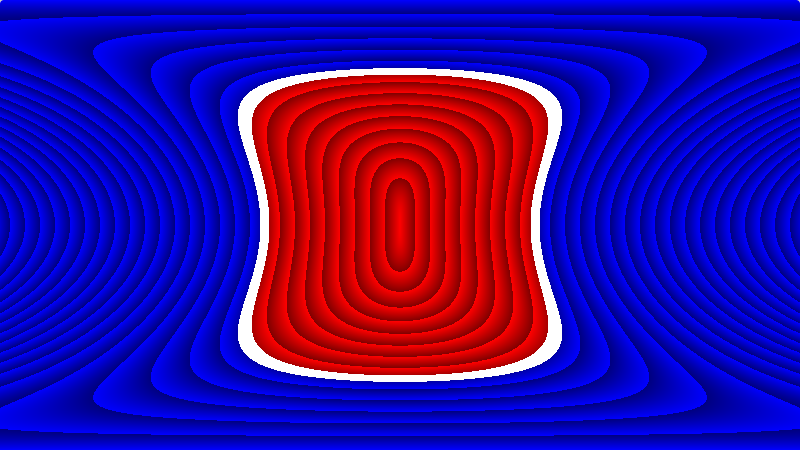
\includegraphics[width=1.0\textwidth]{secciones/imagenes/sdf/2d/sdf_deform.png}\label{fig:deform}
  \caption{Deformación del espacio de una circunsferencia FDS}
\end{figure}

% https://www.shadertoy.com/view/3lsfWj

Las aplicaciones explicadas anteriormente, en general, se extienden a \(\mathbb{R}^3\). Por ejemplo, vamos a ver como primitivas generalizan a las de una dimensión superior.

\section{Primitivas en \(\mathbb{R}^3\)}

\subsection{Esfera exacta}
Esta función es generalizada de la ecuación en 2D, la idea es la misma, aquellas distancias que antes eran positivas con valor \(r\), quedan anuladas al restarles \(r\) y por tanto, forman una \textit{isosuperficie}. En código,
\begin{lstlisting}
// Esfera R3
float SDFEsfera(vec3 p, float r){
    return length(p) - r;
}
\end{lstlisting}
Utilizando el \textit{Marcher} y el \textit{modelo de iluminación de Phong}, el resultado es el observado en la \fullref{fig:phong}.

\subsection{Prisma rectangular exacto}
Este es generalizado del \textit{Rectángulo exacto} en \(\mathbb{R}^2\), el valor absoluto situará las coordenadas en el cuadrante positivo, de los ocho presentes. Las medidas utilizadas serán la mitad, es decir, \(\Vec{s’}= \dfrac{\Vec{s}}{2}\). Aunque no vamos a ver la demostración, una idea de esta es similar a la utilizada para demostrar el rectángulo, cada región exterior de cada cara es anulada, el interior se utiliza la distancia al lado más próximo y en la arista, la distancia euclídea. El resultado.

\begin{lstlisting}
// Prisma R3
float SDFPrisma(vec3 p, vec3 s){
    vec3 pa = abs(p) - s;
    return length(max(pa, 0.)) +
    min(max(max(pa.x, pa.y), pa.z), 0.);
}
\end{lstlisting}

Para la visualización de este resultado, vamos a aplicar una rotación sobre el eje \(YZ\) que lo veremos para \(\mathbb{R}^3\) en la siguiente sección.

\begin{lstlisting}
float escena_sdf(vec3 p){
    // Rotacion plano yz
    vec3 pr = vec3(p.x, p.yz * rot(PI/4.0));
    // Cubo s=0.3 => s'=0.15
    vec3 sp = vec3(0.15);
    return SDFPrisma(pr, sp);
}
\end{lstlisting}

El resultado,
\begin{figure}[H]
  \centering
  \captionsetup{justification=centering}%,margin=2cm
  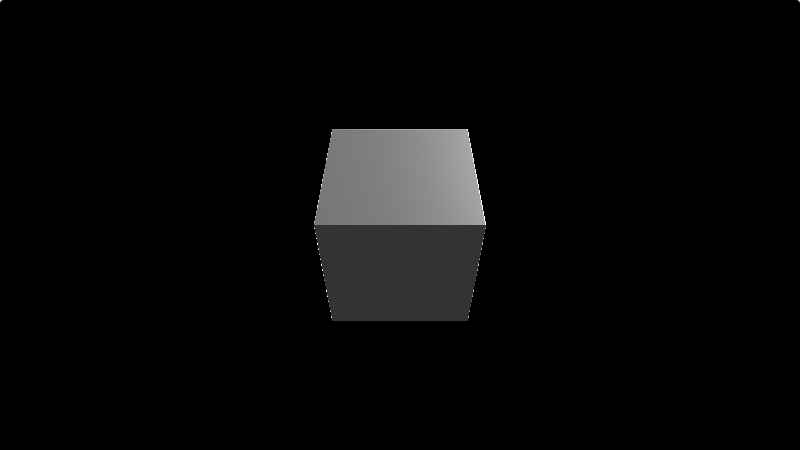
\includegraphics[width=1.0\textwidth]{secciones/imagenes/sdf/3d/sdf_prisma_rect.png}\label{fig:prisma}
  \caption{Prisma Rectangular \(\Vec{s}=\Vec{0.3}\) rotado \(\alpha_{YZ}=\dfrac{\pi}{4}\) FDS}
\end{figure}

% https://www.shadertoy.com/view/WtlBDj

\subsection{Plano con signo}
% TODO: Ordenar el texto de la normal.
Vamos a ver una figura muy importante, el plano con signo divide a \(\mathbb{R}^3\) en dos, uno tendrá valores positivos y el otro, negativos. El signo del producto escalar con la normal del plano indicará en que subespacio se encuentran los puntos. Para esto, definimos el operador del signo de un número:  \(\text{sign}(a)=\pm 1, 0\).\\\\
En secciones siguientes veremos por qué es útil el signo, definiendo así otro operador. Su demostración se basa en la proyección de un punto \(\Vec{p}\) en el plano\footnote{Podemos definir un plano a partir de su normal y un punto, en particular, el punto será \(0,0,0\) y la normal será un parámetro introducido por el usuario. Formalmente lo encontramos en el siguiente enlace \url{https://mathworld.wolfram.com/Plane.html}.}, centrado en el origen y con un vector normal \(\Vec{n}\).
\[\text{proy}_{\Vec{n}}(\Vec{p}) = \Vec{p} - (\Vec{n}\cdot\Vec{p})\Vec{n} \]
Por lo que la distancia con signo a este:
\[ SDFPlano_{\Vec{n}}(\Vec{p})=\text{sign}\left((\Vec{p}-\text{proy}_{\Vec{n}}(\Vec{p})\right) \cdot \Vec{n})\cdot \vert \vert \Vec{p} - \text{proy}_{\Vec{n}}(\Vec{p}) \vert\vert \]
Simplificamos esta ecuación,
\[ SDFPlano_{\Vec{n}}(\Vec{p}) = \text{sign}\left((\Vec{n}\cdot\Vec{p})\Vec{n}\right) \cdot \Vec{n})\cdot \vert \vert (\Vec{n}\cdot\Vec{p})\Vec{n}  \vert\vert \]
Utilizando las siguientes propiedades: \((\Vec{n}k)\cdot\Vec{n}=k\) y \(\vert\vert k\Vec{n}\vert\vert=k\vert\vert\Vec{n}\vert\vert\).
\[ SDFPlano_{\Vec{n}}(\Vec{p})=\text{sign}\left(\Vec{n}\cdot\Vec{p}\right)\cdot (\Vec{n}\cdot\Vec{p}) \vert \vert\Vec{n}\vert\vert=\Vec{n}\cdot\Vec{p}\]

En código,

\begin{lstlisting}
// Plano R3
float SDFPlano(vec3 p, vec3 n){
   return dot(p, n);
}
\end{lstlisting}

Veamos un ejemplo, pero antes, vamos a desplazar el plano hacia abajo, el operador de traslación lo hemos visto en la sección anterior para una diension inferior y veremos que es equivalente para esta dimensión.
\begin{lstlisting}
float escena_sdf(vec3 p){
    // Desplazamiento
    vec3 pt = p - vec3(0., -1., 0.);
    // Plano con normal hacia arriba
    vec3 n = normalize(vec3(0., 1., 0.));
    return SDFPlano(pt, n);
}
\end{lstlisting}

El resultado,

\begin{figure}[H]
  \centering
  \captionsetup{justification=centering}%,margin=2cm
  
\includegraphics[width=1.0\textwidth]{secciones/imagenes/sdf/3d/sdf_plano.png}\label{fig:plano}
  \caption{Plano \(\Vec{n}=(0,1,0)\) desplazado \(\Vec{t}=(0, -1, 0)\)}
\end{figure}

% https://www.shadertoy.com/view/3llBW2

\subsection{Recta y segmento exacto}

Podemos generalizar de la definición vista para la recta en \(\mathbb{R}^2\) para una dimensión superior, así como para la proyección y el segmento.
En código,
\begin{lstlisting}
// Proyección a sobre b
vec3 proy(in vec3 a, in vec3 b){
    return b * dot(b, a) / dot(b, b);
}
// Proyección a sobre b restringido 0, 1
vec3 proy01(in vec3 a, in vec3 b){
    return b * clamp(dot(b, a) / dot(b, b), 0., 1.);
}
// Recta SDF
float SDFRecta(vec3 p, vec3 a, vec3 b){
    vec3 v = p - a;
    vec3 w = b - a;
    return length(v -  proy(v, w));
}
// Segmento SDF
float SDFSegmento(vec3 p, vec3 a, vec3 b){
    vec3 v = p - a;
    vec3 w = b - a;
    return length(v -  proy01(v, w));
}
\end{lstlisting}

\begin{figure}[H]
  \centering
  \captionsetup{justification=centering}%,margin=2cm
  \subfloat[Imagen original]{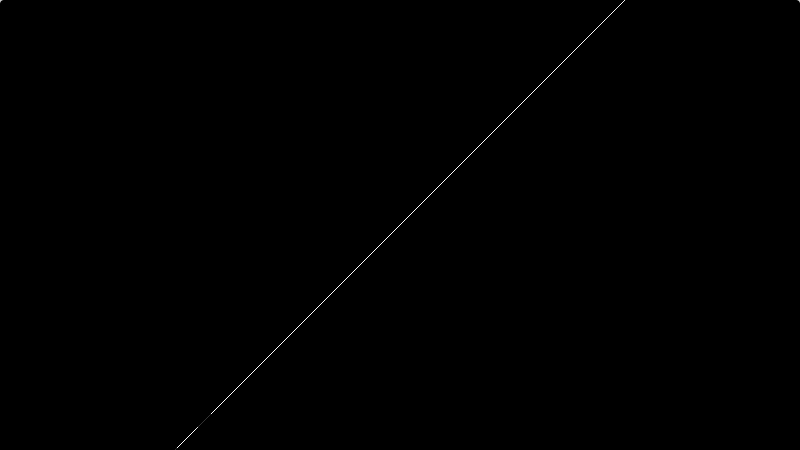
\includegraphics[width=0.45\textwidth]{secciones/imagenes/sdf/3d/sdf_recta_3d.png}\label{fig:recta3d}}
  \hfill
  \subfloat[\(f\) aplicada sobre la imagen original]{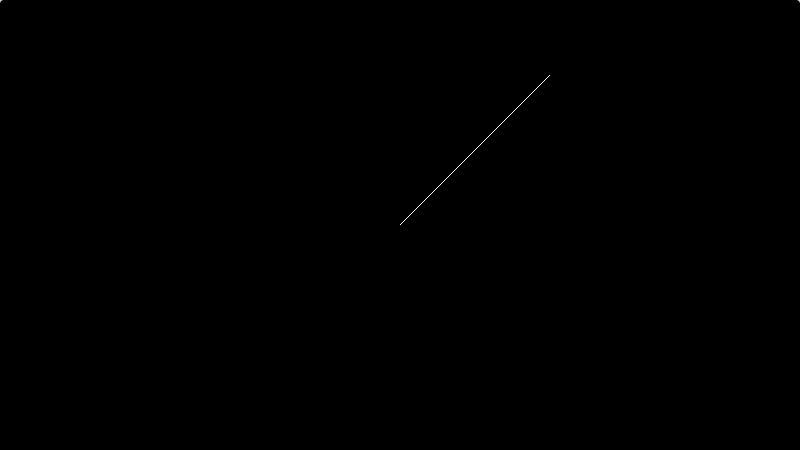
\includegraphics[width=0.45\textwidth]{secciones/imagenes/sdf/3d/sdf_segmento_3d.png}\label{fig:segmento3d}}
  \caption{Recta y Segmento Exacto \(\Vec{a}=\Vec{0}\), \(\Vec{b}=\Vec{0.5}\) SDF}
\end{figure}

% https://www.shadertoy.com/view/3tXBWX 
% https://www.shadertoy.com/view/WtXBWX

Veremos un operador para incrementar el ancho de la recta o del segmento. Algunos de los operadores que vamos a ver también son generalizaciones de los operadores también  vistos en \(\mathbb{R}^2\).

\section{Operadores sobre \(\mathbb{R}^3\)}

\subsection{Operadores Isométricos}
Tenemos a los mismos \textit{Operadores isométricos sobre \(\mathbb{R}^2\)} vistos en secciones anteriores: el operador de traslación, el operador de rotación, el de simetría y el operador de escalado. Se puede demostrar que los operadores son isometrías de manera equivalente a como se demostraron para \(\mathbb{R}^2\).\\\\
Vamos a ver la rotación ya que esta se ha visto sobre el plano \(\overline{XY}=\mathbb{R}^2\) en \(\mathbb{R}^3\). Definimos una rotación sobre cada uno de los tres planos formados por los ejes, tales que:\\\\
Para el plano \(\overline{XY}\), mantenemos la coordenada \(Z\) como libre:
\[\text{rotacion}_{\overline{XY}}^\alpha(\Vec{p}) = \left(x\cos(\alpha) + y\sin(\alpha),-x\sin(\alpha) + y\cos(\alpha),z\right) \]
Para el plano \(\overline{YZ}\), con la coordenada \(X\) como libre:
\[\text{rotacion}_{\overline{YZ}}^\alpha(\Vec{p}) = \left(x, y\cos(\alpha) + z\sin(\alpha),-y\sin(\alpha) + z\cos(\alpha)\right) \]
Finalmente, el plano \(\overline{XZ}\), con la coordenada \(Y\) libre:
\[\text{rotacion}_{\overline{XZ}}^\alpha(\Vec{p}) = \left(x\cos(\alpha) + z\sin(\alpha),y,-x\sin(\alpha) + z\cos(\alpha)\right) \]
Aunque su definición parece bastante compleja, en código es bastante simple de implementar,
\begin{lstlisting}
// Matriz de Rotacion
mat2 rot(float a){
    return mat2(
        +cos(a), -sin(a), 
        +sin(a), +cos(a)
    );
}
// Rotación del plano XY
vec3 rotXY(vec3 p, float a){
    vec2 pr = p.xy * rot(a);
    return vec3(pr.x, pr.y, p.z);
}
// Rotación del plano YZ
vec3 rotYZ(vec3 p, float a){
    vec2 pr = p.yz * rot(a);
    return vec3(p.x, pr.x, pr.y);
}
// Rotación del plano XZ
vec3 rotXZ(vec3 p, float a){
    vec2 pr = p.xz * rot(a);
    return vec3(pr.x, p.y, pr.y);
}
\end{lstlisting}

El resultado de rotar un cubo sobre el plano \(\overline{YZ}\) lo podemos ver en la \fullref{fig:prisma}, con un ángulo \(\alpha=\dfrac{\pi}{4}\).\\\\
Vamos a presentar un operador capaz de incrementar la \textit{isosuperficie} de una figura, similar a como hicimos con la esfera, pudiendo también redondear superficies, que es consecuencia directa de la métrica euclídea.

\subsection{Operador de ensanchamiento}
Presentamos el operador de ensanchamiento, este operador va a crear otras funciones de distancia con signo con mayor superficie, ¿ó menor?. Por ejemplo, puede ser útil en situaciones cuando el marcher no es capaz de trazar la figura debido a la poca superficie, como nos pasa con la recta o el segmento.\\\\
Restaremos un valor \(k\in\mathbb{R}\) a la \textit{isosuperfice}, algunos autores llaman a este operador \enquote{salto de \textit{isosuperficie}}\footnote{Íñigo Quilez utiliza esta terminología en su blog \enquote{Iquilezles} en una de sus entradas: \enquote{3D Distance Functions, Rounding - exact}. El enlace, \url{https://www.iquilezles.org/www/articles/distfunctions/distfunctions.htm}}, aunque también se puede utilizar para \textit{isoperímetros}.\\\\ 
Una idea de la demostración es observar que sobre cualquier punto de una isosuperficie se puede posicionar una esfera cuya superficie es proporcional al radio, la resta de \(k\) sobre las distancias provoca un incremento del radio de la esfera y por tanto, de la superficie.  
\[\text{ensanchar}_k(\Vec{p}, f)=f(\Vec{p})-k\]
Veamos el ensanchamiento del segmento visto en \fullref{fig:segmento3d}, esta nueva función es llamada cápsula.
\begin{lstlisting}
// FDS Cápsula
float SDFCapsula(vec3 p, vec3 a, vec3 b, float k){
	return SDFSegmento(p, a, b) - k;
}
\end{lstlisting}
El resultado es el siguiente,
\begin{figure}[H]
  \centering
  \captionsetup{justification=centering}%,margin=2cm
  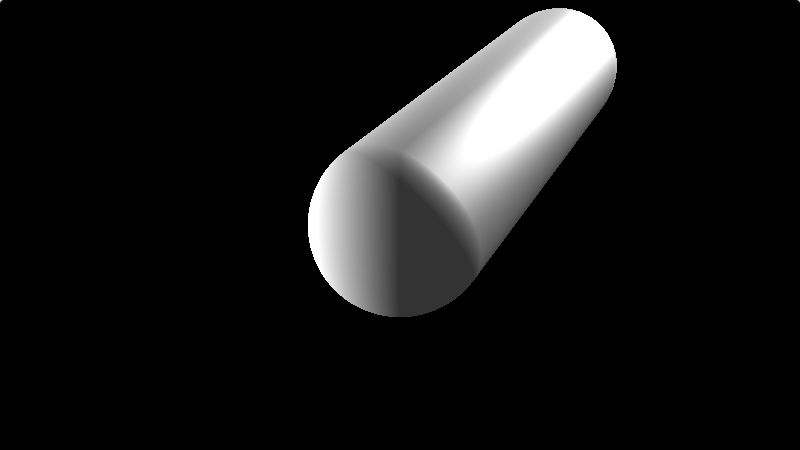
\includegraphics[width=1.0\textwidth]{secciones/imagenes/sdf/3d/sdf_capsula.png}\label{fig:capsula}
  \caption{Segmento ensanchado exacto FDS}
\end{figure}

% https://www.shadertoy.com/view/3tXfDl

Podemos observar que este operador devuelve una figura ensanchada con los bordes redondeados, debido a la métrica, aunque podemos conseguir una figura con bordes redondeados y con la dimensiones originales, sin ensanchar, combinándolo con el operador de escalado.\\\\
Finalmente, vamos a presentar operadores que transforman figuras exactas de \(\mathbb{R}^2\) en otras en \(\mathbb{R}^3\) de manera exacta. Esto nos será útil ya que podemos calcular una \textit{función de distancia con signo exacta} en \(\mathbb{R}^2\) y utilizar uno de estos operadores para crear uno nuevo que deducirlo matemáticamente, hubiera sido tedioso. Vamos a ver dos, el operador de \textit{revolución} y el operador de \textit{extrusión}.
\newpage
%%%%%%%% TODO::::
\subsection{Operador de revolución}
El resultado de este operador es una figura generada por el giro sobre un eje de la figura plana.\\\\
Vamos a calcular la distancia positiva al isoperímetro, dado el plano \(\overline{AB}\) sobre el que está la figura \(f:\mathbb{R}^2\longrightarrow\mathbb{R}\) y dado un punto \(\Vec{p}\in\mathbb{R}^3\) sobre la escena, la proyección de \(\Vec{p}\) sobre el plano \(\overline{AB}\) será \(\Vec{p}_{a,b}\) con \(c\) como coordenada independiente y cuya distancia de la proyección al isoperímetro será \(f(\Vec{p}_{a,b})\), por definición. Si \(\Delta h=(c-0)\) es la altura respecto de \(\Vec{p}\) sobre el plano \(\overline{AB}\), se crea un triángulo equilátero de lados \(\Delta h\) y \( f(\Vec{a,b})\) (Obsérvese la figura \fullref{fig:proof_rev}) y la distancia \Vec{p} hasta el isperímetro de la figura sobre el plano será la diagonal del triángulo formado.
\[\text{distancia}_{\overline{AB}}(\Vec{p}, f)= \sqrt{(\Delta h)^2+(f(\Vec{p}_{a,b}))^2}=\vert\vert(c, f(\Vec{p}_{a,b})\vert\vert\]

Podemos utilizar esta técnica para ensanchar también el isoperímetro trazado para la revolución:

\[\text{revolucion}_{\overline{AB}}^k(\Vec{p}, f)=\text{distancia}_{\overline{AB}}(\Vec{p}, f)-k\]

Veamos un ejemplo de una figura exacta que podemos generar, por ejemplo, un toro\footnote{Se trata de una figura en forma de donut}. La obtenemos de revolucionar una circunsferencia desplazada. En código,

\begin{lstlisting}
/// FDS Toro
float SDFToro(vec3 p, float r1, float r2){
    // FDS Circunsferencia desplazada izq r1 del centro.
    float d = length(p.xz) - r1;
    // Calculamos altura
    float dh = p.y - 0.;
    // Calculamos la distancia (la diagonal)
    return SDFCircunferencia(vec2(dh, d),r2);
}
\end{lstlisting}

\begin{figure}[H]
  \centering
  \captionsetup{justification=centering}%,margin=2cm
  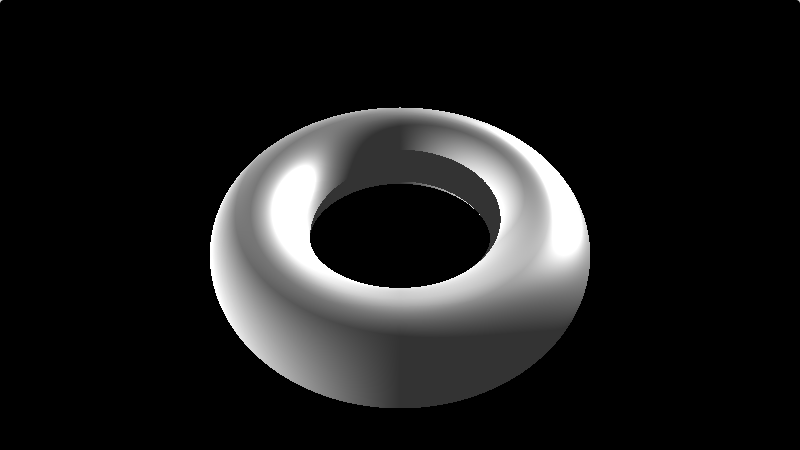
\includegraphics[width=1.0\textwidth]{secciones/imagenes/sdf/3d/sdf_toro.png}\label{fig:torus}
  \caption{Toro exacto por revolución FDS}
\end{figure}

% https://www.shadertoy.com/view/WtsBDf

\subsection{Operador de extrusión}
Este último operador consiste en elongar una figura plana hacia un eje. Pudiendo ser de manera finita o infinita. Cada punto \(\Vec{p}\in\mathbb{R}^3\) se proyecta sobre el plano a extruir y se calcula la función de distancia \(\mathbb{R}^2\). Sea \(\Vec{n}\) el  vector normal del plano de extrusión y \(f\) un \textit{FDS}, el operador se define como:
\[\text{extrusion}^\infty_{\Vec{n}}\left(\Vec{p},f\right) = f\left(\text{proy}_{\Vec{n}}(\Vec{p})\right)\]
En caso de una extrusión finita, de longitud \(h\), definimos como \(\Delta c\) la distancia a la tapadera, haremos uso de la simetría sobre el plano, reduciendo el problema, tal que, la \enquote{altura} será:
\[\Delta c  =\vert\vert \Vec{p} - \text{proy}_{\Vec{n}}(\Vec{p}) \vert\vert - h\]
Dividimos el ejercicio en dos subproblemas, por encima de la tapa \(\Delta c \ge 0\) y aquellas por debajo \(\Delta < 0\). Como referencia, \fullref{fig:proof2}.

\begin{figure}[H]
  \centering
  \captionsetup{justification=centering}%,margin=2cm
  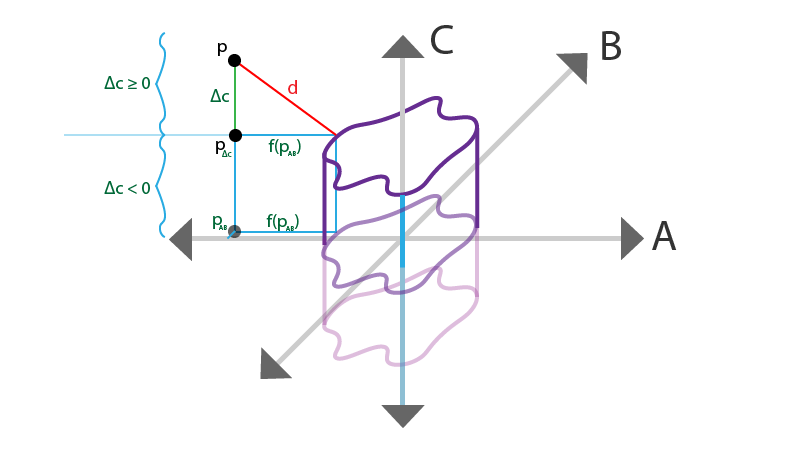
\includegraphics[width=1.0\textwidth]{secciones/imagenes/sdf/proofs/proof_extrussion.png}\label{fig:capsula}
  \caption{Visualización de una extrusión genérica}
\end{figure}

\begin{enumerate}
    \item \textbf{Subproblema 1}. La distancia puede ser negativa o positiva y corresponde con la distancia que devuelve nuesta función \(f\) sobre la proyección del punto en el plano.
    \[d_1=f(\text{proy}_{\Vec{n}}(\Vec{p}))\]
    \item \textbf{Subproblema 2}. Se trata de distancias positivas, observamos en la imagen que se forma un triángulo rectángulo de altura \(\Delta c\) y de base \(f(\text{proy}_{\Vec{n}}(\Vec{p}))\) como el \textbf{Subproblema 1}. La diagonal \(d\) corresponde a la distancia de \(\Vec{p}\) a la superficie de la tapadera.
    \[d_2=\sqrt{(\Delta c)^2+f(\text{proy}_{\Vec{n}}(\Vec{p}))^2}\]
\end{enumerate}

Veamos como podemos unificar ambos subroblemas como hicimos con el rectángulo. Cuando \(\Delta c < 0\), queremos que \(d_1=d_2\), esto se consigue haciendo que \(\Delta c\) sea 0 cuando este sea negativo,
\[d_2=\sqrt{\max(\Delta c, 0)^2+d_1^2}=\vert\vert (\max(\Delta c, 0), d_1)\vert\vert\]

Vamos a generar el interior y exterior de la figura, los cuales se anularán con independencia. Por eso, \(d_2\) se anulará cuando el punto esté en el interior. Para ello, en la ecuación, \(d_1\) debe anularse cuando este sea negativo.
\[d_{exterior}=\vert\vert (\max(\Delta c,0), \max(d_1, 0))\vert\vert\]

El interior de la figura ocurre cuando \(\Delta c < 0\) y \(d_1 < 0\), por lo que se anularán cuando sean positivos. Tomaremos el máximo de las dos distancias para encontrar la mínima negativa.
\[d_{interior} = \text{argmax}(\Delta c, d_1) = \min(\max(\Delta c, f(\text{proy}_{\Vec{n}}(\Vec{p})), 0)\]
Finalmente, como se anulan, podemos sumar y la ecuación resultante será:
\[\text{extrusion}^h_{\Vec{n}}\left(\Vec{p},f\right)=\vert\vert \max((\Delta c, d_1), 0)\vert\vert +  \text{argmax}(\Delta c, d_1) \]

Un ejemplo de esta técnica es la fabricación del cilindro exacto con y sin tapa de radio \(r\). En código:
\begin{lstlisting}
// Proyección sobre plano
vec3 proyPlano(vec3 p, vec3 n){
    return p - dot(p, n) * n;
}
// FDS circunsferencia
float SDFCircunferencia(vec2 p, float r){
	return length(p) - r;
}
// FDS Cilindro
float SDFCilindro(vec3 p, float r){
    // Proyeción sobre el plano YZ => n = X
    vec3 n = normalize(vec3(1, 0, 0));
    // Cogemos el plano YZ
    vec2 proy = proyPlano(p, n).yz;
    // Devolvemos la circunsferencia
    return SDFCircunferencia(proy, r);
}
// FDS Cilindro Finito (Con Tapa)
float SDFCilindro(vec3 p, float h, float r){
    // Proyeción sobre el plano YZ => n = X
    vec3 n = normalize(vec3(1, 0, 0));
    // Calculamos la proyección
    vec3 proy = proyPlano(p, n);
    // Altura sobre la tapa.
    float dc = length(p - proy) - h;
    // FDS Circunferencia de radio r sobre la proyección en el plano YZ.
    float fproy = SDFCircunferencia(proy.yz, r);
    // Exterior figura
    float dint = length(max(vec2(dc,fproy),0.));
    // Interior de la figura
    float dext = min(max(dc, fproy), 0.);
    // Sumamos ambos
    return dint + dext;
}
\end{lstlisting}

Dibujaremos una circunsferencia en el plano \(\overline{YZ}\) y extruiremos utilizando el vector normal \(\Vec{n}=(0,0,1)\) infinitamente, en el segundo, de longitud \(h=0.6\).

\begin{figure}[H]
  \centering
  \captionsetup{justification=centering}%,margin=2cm
  \subfloat[Cilindro sin tapa]{
\includegraphics[width=0.45\textwidth]{secciones/imagenes/sdf/3d/sdf_cilindro_infinito.png}\label{fig:cilindro_inf}}
  \hfill
  \subfloat[Cilindro con tapa]{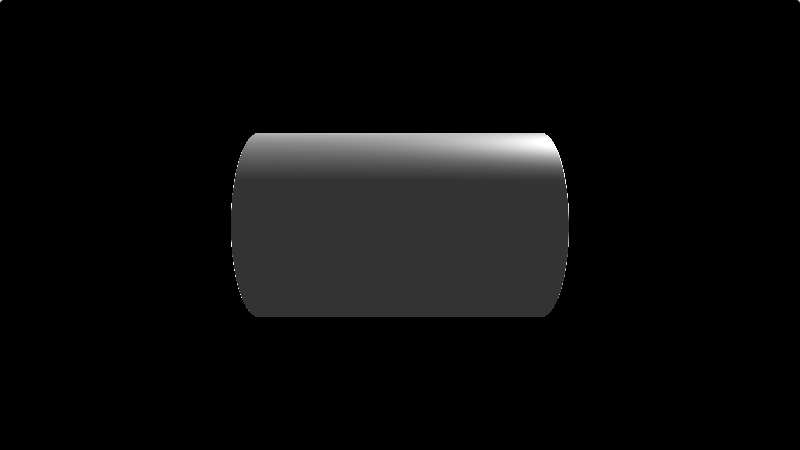
\includegraphics[width=0.45\textwidth]{secciones/imagenes/sdf/3d/sdf_cilindro.png}\label{fig:cilindro_tapa}}
  \caption{Cilindro exacto por extrusión con \(r=0.2\) y \(h'=0.3\)  FDS}
\end{figure}

% https://www.shadertoy.com/view/3lsfDX
% https://www.shadertoy.com/view/3tlBWf

\subsection{Operador de agregación y substracción}
Vamos a recordar los operadores de agregación y de substracción presentados anteriormente, en la sección de operadores en \(\mathbb{R}^2\) y que son equivalentes para \(\mathbb{R}^3\). Vamos a presentar también un nuevo operador, el operador de sección en el que utilizaremos el plano con signo, visto anteriormente. Para el primer ejemplo, vamos a utilizar dos esferas con el mismo radio y una separada de la otra. El código de la agregación será:
\begin{lstlisting}
float escena_sdf(vec3 p){
    // Dos esferas, una trasladadas
    // Agregacion
    return min(
        SDFEsfera(p, 0.3),
        SDFEsfera(p - vec3(0.3, 0., 0.), 0.3)
    );
}
\end{lstlisting}
su resultado:
\begin{figure}[H]
  \centering
  \captionsetup{justification=centering}%,margin=2cm
  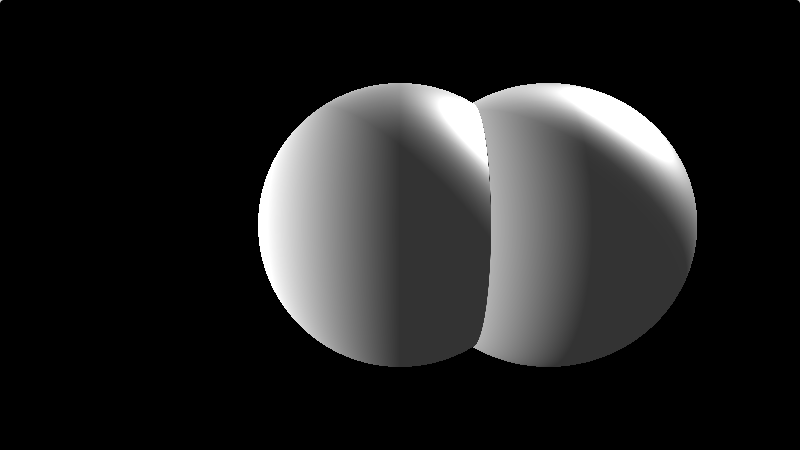
\includegraphics[width=1.0\textwidth]{secciones/imagenes/sdf/3d/sdf_add_3d.png}\label{fig:add3d}
  \caption{Agregación de dos esferas \(r=0.3\) y una trasladada}
\end{figure}

% https://www.shadertoy.com/view/3llBWl

Como ya se ha comentado, el operador \enquote{\(\max\)} devuelve la intersección de ambas figuras. Vamos a utilizar la definición del plano con signo para seccionar una figura, ya que una región es sólida y la otra no. \\\\

\begin{lstlisting}
float escena_sdf(vec3 p){
    // Rotamos el plano XZ, pi / 4 rad
    p = rotXZ(p, PI / 2. * 1.2);
	// Sección de una esfera
    return max(
        SDFEsfera(p, 0.3),
        SDFPlano(p - vec3(0., 0., 0.15), vec3(0., 0., 1.))
    );
}
\end{lstlisting}

Se trata de una sección del eje \(\Vec{z}\), desplazando el plano con el operador de traslación con \(\Vec{t}=(0,0,0.3)\), pudiendo así modificar la posición de la sección. El resultado es el siguiente:

\begin{figure}[H]
  \centering
  \captionsetup{justification=centering}%,margin=2cm
  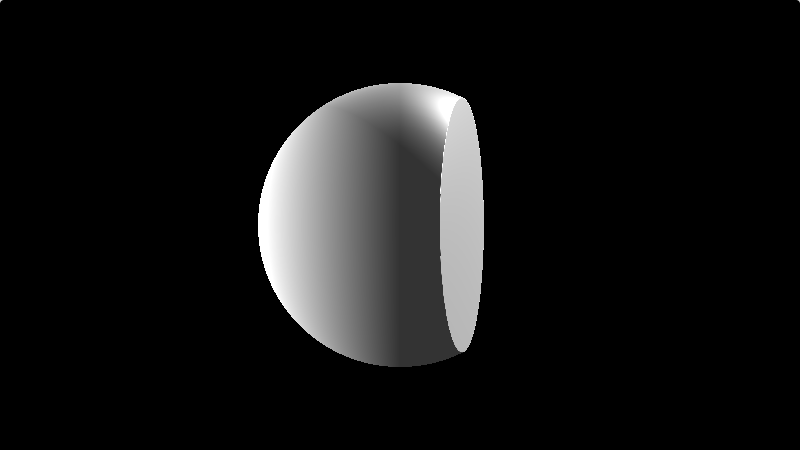
\includegraphics[width=1.0\textwidth]{secciones/imagenes/sdf/3d/sdf_seccion_3d.png}\label{fig:seccion}
  \caption{Una esfera \(r=0.3\) seccionada por un plano \(\Vec{n}=(0,0,-1)\) desplazado}
\end{figure}

% https://www.shadertoy.com/view/WtsBWl

Finalmente, veamos un ejemplo de \textit{subtracción}, utilizando las dos esferas vistas antes. En código:

\begin{lstlisting}
float escena_sdf(vec3 p){
    // Rotamos el plano XZ, pi / 4 rad
    p = rotXZ(p, PI / 4.);
    // Substraccion b en a => max(a, -b)
    return max(
        SDFEsfera(p, 0.3),
        -SDFEsfera(p - vec3(0.3, 0., 0.), 0.3)
    );
}
\end{lstlisting}


Rotaremos la escena para poder ver así el interior, utilizaremos el operador de rotación del plano \(\overline{XZ}\) con \(\alpha=\dfrac{\pi}{4}\). El resultado será una esfera en el centro a la que se le ha carvado otra esfera, trasladada:

\begin{figure}[H]
  \centering
  \captionsetup{justification=centering}%,margin=2cm
  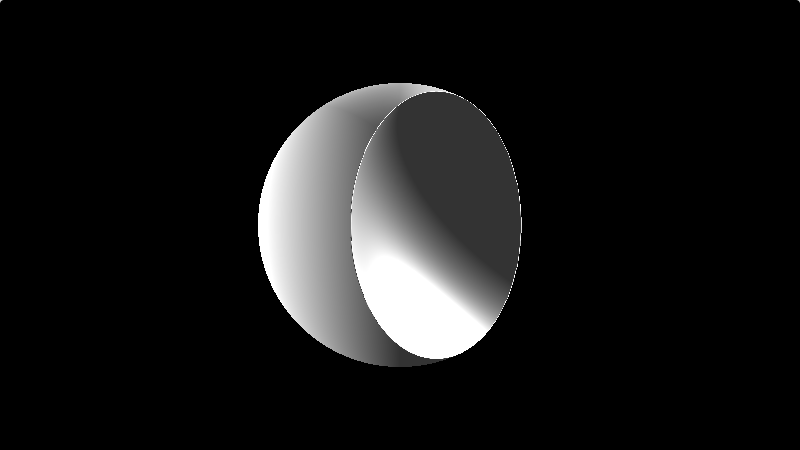
\includegraphics[width=1.0\textwidth]{secciones/imagenes/sdf/3d/sdf_substract_3d.png}\label{fig:sub3d}
  \caption{Dos esferas \(r=0.3\) y substracción de la trasladada}
\end{figure}

% https://www.shadertoy.com/view/WlsBWl

\subsection{Operador de deformación no exacta}
Veamos el último operador el de deformación, recordemos que este no siempre conserva la métrica, provocando lo que llamaremos \enquote{artefactos}. En la siguiente sección veremos como resolverlos. Vamos a definir la siguiente deformación contínua y derivable:
\[g(\Vec{p})=(
\Vec{p}_x \cos(10\Vec{p}_y) + \Vec{p}_z\sin(10\Vec{p}_y),
\Vec{p}_y,
\Vec{p}_x\sin(10\Vec{p}_y) + \Vec{p}_z\cos(10\Vec{p}_y)
)
\]
Esta deformación es conocida como \textit{torsión}, consiste en rotar un eje, o plano, a medida que incrementa la distancia a este. Utilizaremos un cubo para este ejemplo, en código:

\begin{lstlisting}
float escena_sdf(vec3 p){
    // Rotamos la escena
    vec2 ry = p.yz * rot(PI / 4.0);
    p = vec3(p.x, ry.x, ry.y);
    // Deformación "g"
    float k = 10.0; // periodo.
    float a = p.y * k;
    p = vec3(
    	+p.x * cos(a) + p.z * sin(a),
    	+p.y,
        -p.x * sin(a) + p.z * cos(a)
    );
	// Dibujamos un prisma.
    return SDFPrisma(p, vec3(0.2));
}
\end{lstlisting}

El resultado obtenido es el siguiente:

\begin{figure}[H]
  \centering
  \captionsetup{justification=centering}%,margin=2cm
  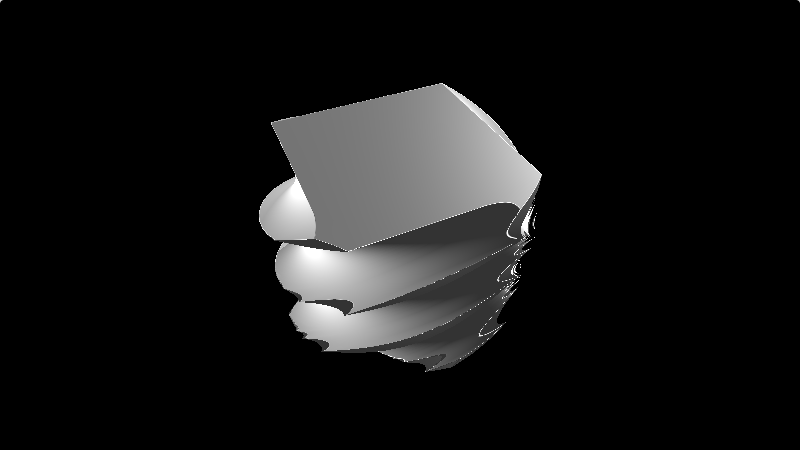
\includegraphics[width=1.0\textwidth]{secciones/imagenes/sdf/3d/sdf_twist.png}\label{fig:twist}
  \caption{Deformación torsión de un cubo \(\Vec{l}=\Vec{0.2}\)}
\end{figure}

% https://www.shadertoy.com/view/ttlfWl

Como vemos, esta deformación ha creado artefactos, por ejemplo, la tapadera es no es completamente cuadrada y vemos que se ha deformado. Esto ocurre ya que la bola también ha sido deformada y esta ahora puede contener algún punto en su interior, sobreestimando.